%%%%%%%%%%%%%%%%%%%%%%%%%%%%%%%%%%%%%%%%%
% Vertical Line Title Page 
% LaTeX Template
% Version 1.0 (27/12/12)
%
% This template has been downloaded from:
% http://www.LaTeXTemplates.com
%
% Original author:
% Peter Wilson (herries.press@earthlink.net)
%
% License:
% CC BY-NC-SA 3.0 (http://creativecommons.org/licenses/by-nc-sa/3.0/)
% 
% Instructions for using this template:
% This title page compiles as is. If you wish to include this title page in 
% another document, you will need to copy everything before 
% \begin{document} into the preamble of your document. The title page is
% then included using \titleGM within your document.
%
%%%%%%%%%%%%%%%%%%%%%%%%%%%%%%%%%%%%%%%%%

%----------------------------------------------------------------------------------------
%	PACKAGES AND OTHER DOCUMENT CONFIGURATIONS
%----------------------------------------------------------------------------------------

\documentclass{article}

\usepackage{pslatex}
\usepackage{listings}
\usepackage{url}
\usepackage{graphicx}


\newcommand*{\plogo}{\fbox{$\mathcal{PL}$}} % Generic publisher logo

%----------------------------------------------------------------------------------------
%	TITLE PAGE
%----------------------------------------------------------------------------------------

\newcommand*{\titleGM}{\begingroup % Create the command for including the title page in the document
\hbox{ % Horizontal box
\hspace*{0.2\textwidth} % Whitespace to the left of the title page
\rule{1pt}{\textheight} % Vertical line
\hspace*{0.05\textwidth} % Whitespace between the vertical line and title page text
\parbox[b]{0.75\textwidth}{ % Paragraph box which restricts text to less than the width of the page

{\noindent\Huge\bfseries The Manual for \\[0.5\baselineskip] ``Native or Not''}\\[2\baselineskip] % Title
{\large \textit{A Project for CS385}}\\[4\baselineskip] % Tagline or further description
{\Large \textsc{Jiaming Shen \\}} % Author name
{\Large \textsc{Zhaowei Tan \\}} % Author name
{\Large \textsc{Zhichen Wu \\}} % Author name

\vspace{0.5\textheight} % Whitespace between the title block and the publisher
{\noindent Shanghai Jiao Tong University \\ IEEE Honor Class}\\[\baselineskip] % Publisher and logo
}}
\endgroup}

%----------------------------------------------------------------------------------------
%	BLANK DOCUMENT
%----------------------------------------------------------------------------------------












\begin{document}

\thispagestyle{empty}
\titleGM % This command includes the title page

%% Generate contents etc
\tableofcontents

\newpage

%% These include the actual text

\section{Introduction}
\paragraph{}
Hello there! Thank you for voting for us and welcome to our project! We are   \textbf{\emph{Team JeeQee O'ye}}, constituted by three people: \textbf{\emph{Jiaming Shen}}, \textbf{\emph{Zhaowei Tan}} and \textbf{\emph{Zhichen Wu}}. 

In this section, we will give a brief introduction on our project, including why we came up with the idea, the expected goal of this project and the practical significance of the work.


\subsection{Motivation}
\paragraph{}
Many of us will apply for graduate schools in the near future. TOEFL score is indespensible for this process, and a higher TOEFL score may increase your chances of being admitted. However, Chinese students tend to earn a low score in Speaking Task, which prohibits some top students from reaching the minimum requirements of their dream schools. 

From this point, we developed our idea. We aim to build a system, via machine learning methods, to help us train the accent in order to achieve a higher TOEFL score. Considering that this goal is way too far from us, we start from a simple task, which will be described in the next subsection.


\subsection{The Basic Goal}
\paragraph{}
Our basic goal is a binary classification problem:
\begin{quote}\textbf{\emph{
	Given a recording of a fixed script of English words, we would like to predict whether the speaker is a native English speaker or not.}}
\end{quote}

There exist some potential advanced tasks, which will be discussed in the later section.


\subsection{Significance}
Upon the finishing the project, the outcome can be used to:
\begin{itemize}
	\item assess your accent
	\item judge the native language
\end{itemize}
The function will be useful for the following people:
\begin{itemize}
	\item ESL teachers and students
	\item People (like actors) who need to learn an accent
	\item Linguists who do research in this area
	\item Computers whose services differ due to native language
	\item Anyone who finds this interesting
\end{itemize}



\newpage


\section{The Dataset}
\subsection{Source of the Data}
\paragraph{}
The recordings are scraped from the George Mason University Department of English Speech Accent Archive \emph{(http://accent.gmu.edu/)}. We do not own the data, and all the credits of the data go to that entity.
\subsection{The Discription of the Data}
\paragraph{}
In the website, all the recordings are classified according to the speakers' native languages.

\begin{figure}[ht]
\begin{center}
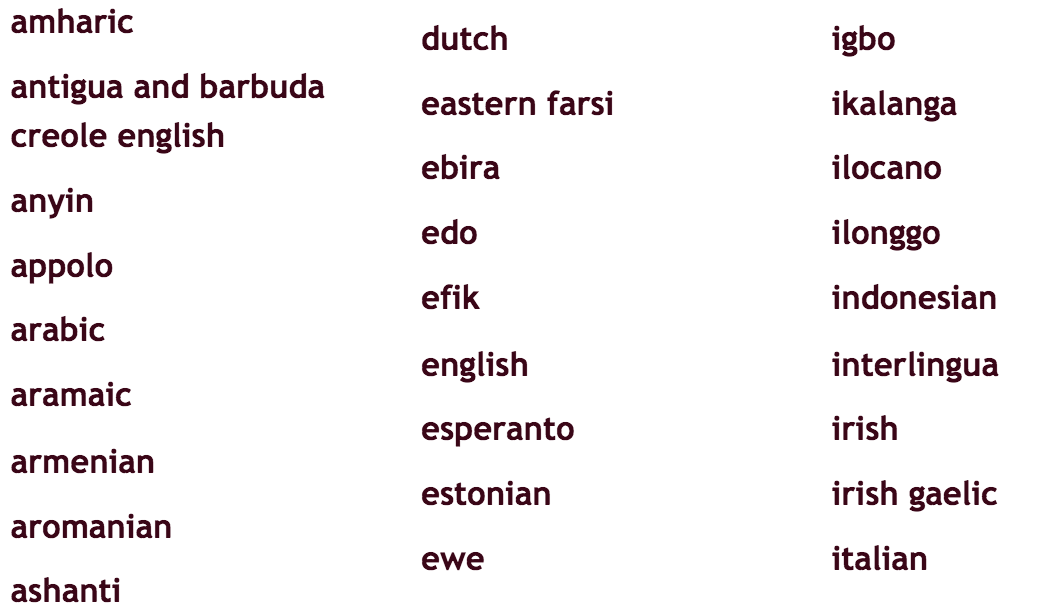
\includegraphics[width=10cm]{classification.png}
\end{center}
\caption{The snapshot of the website}
\end{figure}

We now have crawled the recordings of two categories, \emph{English} and \emph{Mandarin}, combing 620 clips together. More categories can be crawled by yourself further, which will be elaborated in Section 2.3.

In each recording, every speaker will read the same English script:
\begin{quote}\emph{
Please call Stella. Ask her to bring these things with her from the store: Six spoons of fresh snow peas, five thick slabs of blue cheese, and maybe a snack for her brother Bob. We also need a small plastic snake and a big toy frog for the kids. She can scoop these things into three red bags, and we will go meet her Wednesday at the train station.}
\end{quote}

In addition to the recording, we scrap the basic information of the speaking, including the native language, birth place (pinpointed to the province), other language spoken, age, sex, age of starting learning english, learning method, english residence (if has, the length of the residence). These data are collected into csv files which have been provided together with the recordings. You can read them using various programming languages.

\begin{figure}[ht]
\begin{center}
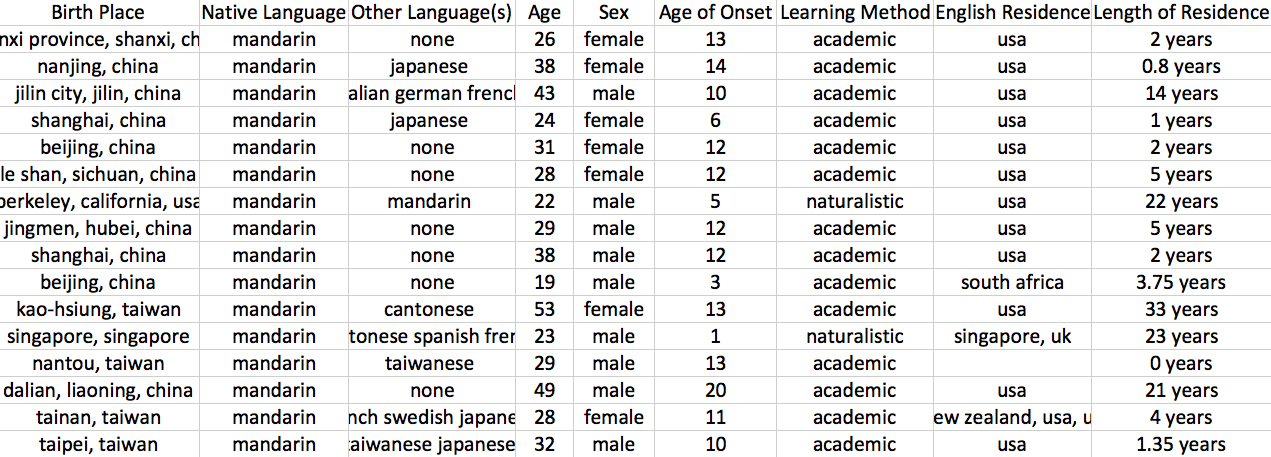
\includegraphics[width=10cm]{csv.png}
\end{center}
\caption{The snapshot of the csv file}
\end{figure}


\subsection{The Crawler}
\paragraph{}
We have provided our own crawler. Given that the number of recordings is lopsided between Mandarin and Native English, you can modify the crawler to get more recordings from other mother languages and use that as your non-native English dataset.

Two crawlers play different roles. \textbf{\emph{music.py}} crawls the recording file, while \textbf{\emph{metadata.py}} crawls the metadata of the speaker. You can modify them to get your dataset.

You can browse different languages in \emph{http://accent.gmu.edu/browse\_language.php}. After your choosing one, you can paste the language name (e.g. arabic) to replace \textbf{\emph{the first ``english''}} in the 5th line of \textbf{\emph{music.py}} and the \textbf{\emph{``english''}} in 15th line of \textbf{\emph{metadata.py}}.

After designating the source of the data, you can change the file name by altering \textbf{\emph{the third ``english''}} in the 5th line of \textbf{\emph{music.py}} and the \textbf{\emph{``english''}} in the 89th line of \textbf{\emph{metadata.py}}.

Finally, do not forget to change the target path where you store the data. The csv file will be store in the same directory by default and you can as well alter \textbf{\emph{the second ``english''}} in the 5th line of \textbf{\emph{music.py}} to change you folder to store the recordings.

\newpage



\section{How to Start}
\paragraph{}
In this section, we present a simple documentation of our startup codes, including the methods of importing data, compressing audioes(optional), and using mfcc to extract features. 

\subsection{Directionary Structure}
-- Start Codes

	--- English
	
	------ english1.wav
		
	------ english2.wav
		
	------ ...
		
	--- Mandarin
	
	------ mandarin1.wav
		
	------ mandarin2.wav
		
	------ ...
		
	--- main.m
	
	--- readData.m
	
	--- compressData.m
	
	--- featureExtract.m
	
	--- readme.md

\subsection{Components}

\begin{itemize}
	\item \textbf{\emph{readData.m}}
	
	First, you should put all your data in a separate foler and name them in a structural and meaningful way. You can import and store all data in a cell array by giving the name of that folder, the specific type of your audioes (`mandarin', `english', etc), as well as their suffix (`.mp3' or `.wav'). 
	
	\item \textbf{\emph{compressData.m}}
	
	This part converts auidoes into sound tracks of approximately the same length. We do this for the sake of later feature extraction part, however, this part is totally optional. We are not sure whether this step will alter some important features of original data, and thus if you are afraid of its possible side effects and want to skip this part, be my guest.
	
	\item \textbf{\emph{featureExtract.m}}
	
	This part use `melfcc.m' in `rastamat' toolbox, so You MUST add `rastamat' directionary into the working path. The input of `melfcc.m' is waveform `x', its sampling rate `fs', and a lot of optional parameters. For more detailed information of `rastamat' toolbox, see resource-1. Besides, we provide a basic tutorial of mfcc, see resource-2.

	P.S. For the baseline system, we use Matlab neural-network toolbox, and for its tutorial please refer to Section 4.1.
	
	
	
\end{itemize}

\newpage

\section{Some Tips}
\subsection{Additional Resources}
\paragraph{}
You can harness the following information to finish this projects:
\begin{itemize}
	\item Rastamat toolbox documentation
	
	\emph{http://labrosa.ee.columbia.edu/matlab/rastamat/}
	
	\item MFCC tutorial
	
	\emph{http://practicalcryptography.com/miscellaneous/machine-learning/guide-mel-frequency-cepstral-coefficients-mfccs/}
	
	\item Matlab neural-network toolbox tutorial
	
	\emph{http://cn.mathworks.com/help/nnet/gs/fit-data-with-a-neural-network.html}
	
	\item The Munich Automatic Segmentation System MAUS
	
	\emph{http://www.bas.uni-muenchen.de/Bas/BasMAUS.html\#downloads}
	
\end{itemize}



\subsection{Advanced Tasks}
\paragraph{}
Here are some advanced version of this project:
\begin{itemize}
	\item Instead of judging native or not, we can judge which the native language of the speaker is, thus presenting a multi-classification problem.
	\item We can using the recordings to predict the onset learning year of the speaker, which stands a regression problem.
	\item Moreover, we can extract the vowels and the consonants in the recordings and use that to predict native or not in any given recordings, breaking the shackles of a given paragraph.
\end{itemize}


\subsection{Contact}
\paragraph{}
If you have any problems or suggestions, you are more than welcomed to contact us. You can either find us in class, or send us e-mails. Please mail to tanzw94@gmail.com.

Thank you again. Enjoy machine learning!





\end{document}